\section{Introduction}\label{sec:introduction}
Antineutrino monitoring has matured from a physics demonstration into a safeguards-relevant sensing modality because the signal is weakly shieldable, physically tied to fissile evolution, and now measurable with higher spectral and temporal fidelity than early deployment studies assumed \citep{SRC035,SRC034,SRC023,SRC018,SRC009,SRC001}. At the same time, fusion-adjacent fuel-cycle pathways have reopened an old but unresolved question: whether material and blanket choices that alter neutron economy can be detected early enough to constrain covert fissile production scenarios under realistic detector noise and calibration drift \citep{SRC007,SRC010,SRC019,SRC025,SRC026,SRC028,SRC036}. The practical issue is not whether one can separate idealized signal classes in simulation; the issue is whether operational false-alarm control, delay, and transfer stability survive contradictory source priors and nuisance misspecification in the regimes where decisions are made.

This work studies that operational regime. We treat detector efficiency, background level, energy resolution, and standoff as explicit nuisance quantities; we keep reactor and fusion-adjacent settings open and parameterized; and we evaluate detection performance under matched false-alarm operating points so comparator differences are not driven by threshold mismatch. The manuscript is intentionally hybrid: it combines formal guarantees for the calibration and ranking operators with executed simulation evidence and symbolic theorem checks. This combination is necessary because purely empirical gains can be unstable under prior contradiction, while purely formal guarantees can fail to capture transfer degradation in high-drift conditions.

The broader relevance extends beyond one safeguards niche. The methodological pattern, namely contradiction-aware prior families, minimax threshold calibration, and explicit robustness accounting, is applicable to other domains that combine sparse physics observability with high-consequence early warning decisions, including process monitoring and infrastructure anomaly detection under domain shift. In that sense, this manuscript contributes both a domain-specific antineutrino result and a generalizable uncertainty-governed detection design template.

Our contributions are:
\begin{itemize}
\item We define a contradiction-aware robust threshold operator for sequential antineutrino detection and prove existence with conservative false-alarm control under explicit regularity assumptions.
\item We derive an information-decomposed minimum detectable diversion criterion showing when joint count-shape inference strictly improves detectability over count-only information.
\item We formalize a finite robust detector-material co-design objective with a stability functional and prove optimizer existence plus bounded stability score.
\item We execute a CPU-feasible benchmark over 17,280 runs across prior families, drift regimes, standoff distances, and detector resolutions, with matched-false-alarm comparator policy and bootstrap uncertainty.
\item We report claim-wise support status with negative-result logging: one core detectability claim is supported, while calibration and transfer-stability claims remain conditional and are bounded by explicit caveats.
\end{itemize}

The evidence summary is concrete. At matched operating points, the robust method improves delay substantially in most regimes (delay win rate $0.9965$ and median delay ratio $0.6943$ against a fixed-threshold test-statistic comparator), but calibration robustness remains incomplete (calibration violation rate $0.9524$, leave-one-prior-out FAR inflation $p95=1.287$), and worst-case transfer degradation is elevated (hard-over-easy ratio $1.540$). Symbolic checks for the theorem-critical algebraic and monotonicity constraints all pass ($4/4$). These combined results motivate a bounded conclusion: robust detectability gains are credible under the tested open-parameterized assumptions, but policy-grade calibration and transfer closure require targeted follow-up experiments.

\section{Related Work and Novelty Boundary}\label{sec:related_work}
\subsection{Reactor Spectrum Baselines and Anomaly Tensions}
Modern reactor antineutrino baselines are anchored by high-statistics flux and spectrum measurements, especially recent Daya Bay analyses and related instrumentation programs \citep{SRC002,SRC003,SRC012,SRC013,SRC014}. These studies improved precision and clarified how isotopic evolution and detector calibration shape inferred spectra. At the same time, anomaly-centered literature emphasizes unresolved model discrepancy across conversion and aggregate-beta pipelines \citep{SRC005,SRC015,SRC029,SRC030,SRC031}. The agreement is strong on one point: isotope fractions and detector systematics materially influence predicted observables. The disagreement remains consequential: competing anomaly attributions imply different prior families and therefore different thresholds for controlling false alarms under misspecification.

Our approach adopts this contradiction as a first-class design input rather than suppressing it. Instead of choosing a single prior lineage, we use a bounded prior family and calibrate for robust control. This differs from common single-prior detector tuning and is the primary formal bridge from anomaly debates to operational alarm design.

\subsection{Safeguards Detection and Sequential Decision Rules}
Operational safeguards studies established that antineutrino streams can track reactor state changes and support diversion-sensitive inference under explicit nuisance handling \citep{SRC035,SRC034,SRC023,SRC022,SRC018,SRC017,SRC011,SRC009,SRC001}. Methodologically, likelihood-ratio and sequential detection frameworks are recurrent, often with count-dominant statistics and site-specific assumptions. More recent analyses show that spectral information can improve discrimination when calibration is controlled \citep{SRC009,SRC017,SRC023}. However, the magnitude and persistence of gains vary with background drift, resolution, and transfer regime, and not all studies enforce comparator fairness through matched false-alarm targets.

This manuscript contributes an explicitly matched operating-point comparison protocol and a claim-evidence closure strategy that separates supported gains from conditional ones. That distinction is important because apparent improvements can disappear once threshold mismatch is removed.

\subsection{Burnup Uncertainty and Fusion-Adjacent Transfer}
Burnup-aware analyses and isotopic evolution studies provide the mechanistic basis for time-varying signal formation \citep{SRC006,SRC008,SRC014,SRC015,SRC021,SRC027,SRC001}. In parallel, fusion and hybrid blanket studies characterize material-dependent breeding pathways and neutron-economy effects that are relevant to covert production risk \citep{SRC007,SRC010,SRC019,SRC025,SRC026,SRC028,SRC033,SRC036}. The central limitation is data realism: many fusion-adjacent studies are conceptual or parameterized, whereas safeguards deployment evidence is largely reactor-domain specific.

The novelty boundary of this paper is therefore precise. We do not claim plant-specific predictive validity for proprietary fusion operations. We claim a reproducible, open-parameterized framework that can rank and stress-test detector-material strategies while preserving explicit caveats on external validity. This boundary is scientifically defensible and prevents over-interpretation.

\subsection{Gap Statement}
Prior literature leaves three linked gaps that motivate this work. First, there is no unified calibration theorem for contradiction-aware prior families integrated with operational FAR constraints. Second, many detectability claims rely on empirical separation without a formal criterion that attributes gains to count and shape information channels. Third, co-design recommendations are frequently nominal and lack explicit robustness objectives with stability auditing under drift. The technical core of this manuscript addresses exactly these gaps while preserving source lineage at each borrowed formal component.

\section{Research Questions and Evaluation Logic}\label{sec:research_questions}
This manuscript is organized around three research questions that follow directly from the contradiction map and the operational safeguards objective. First, can contradiction-aware calibration preserve false-alarm control while retaining delay performance? Second, does adding shape information produce meaningful detectability gains under matched operating points and nuisance propagation? Third, can detector-material co-design maintain performance when moving from easier to harder nuisance regimes? The questions are linked; answering only one is not sufficient for reliable monitoring guidance.

The first question concerns calibration reliability under model disagreement. Prior work often uses a single emission lineage or reports thresholding details incompletely, which makes false-alarm comparisons difficult across studies. By explicitly defining a bounded prior family and evaluating leave-one-prior-out stress, we turn disagreement into a measurable robustness objective instead of an untracked uncertainty source. This design choice is motivated by anomaly and conversion-model tensions in the reactor literature and is essential for transfer-minded safeguards analysis \citep{SRC005,SRC015,SRC029,SRC030,SRC031}.

The second question concerns mechanistic detectability, not only headline metrics. Count-only improvements can occur for reasons unrelated to material signatures, for example due to threshold mismatch or favorable background slices. The information-decomposed MDS criterion in this manuscript was introduced to avoid that ambiguity. It asks whether shape information contributes positive information under the same FAR target and nuisance treatment, which is a sharper question than asking whether one method has a smaller median delay in aggregate.

The third question concerns deployment stability. A method that performs well in nominal settings but degrades strongly under drift and standoff variation can be scientifically interesting yet operationally fragile. We therefore evaluate robust co-design through worst-regime scalarization and a bounded stability diagnostic. This emphasizes resilience over isolated peak performance and aligns with safeguards use where conditions can change faster than recalibration cycles.

\subsection{Comparator Philosophy}
Comparator selection in this study follows a lineage-aware philosophy. We include methods that represent common operational families: single-prior likelihood ratio, count-only sequential testing, nuisance-penalized spectral fit, fixed-threshold test-statistic detection, and FAR-matched CUSUM. This set is deliberately heterogeneous. It allows us to test whether gains from contradiction-aware calibration persist relative to both classical count-focused methods and spectral-statistical alternatives discussed in modern monitoring studies \citep{SRC035,SRC034,SRC023,SRC022,SRC018,SRC017,SRC009,SRC001}.

Matched operating-point policy is central to fair comparison. Without matching, a method can appear superior by accepting higher false-alarm burden. Because operational burden is itself a mission variable, mismatched comparisons are not informative for safeguards design. All primary claims in this manuscript therefore depend on matched-FAR evaluation, and claims are downgraded when stress criteria fail even if nominal delay gains are large.

\subsection{What Counts as Evidence in This Paper}
Evidence is stratified into four layers. The first layer is source-grounded formalism: reused equations and assumptions from the acquired corpus. The second layer is manuscript-defined formal extension: threshold, MDS, and co-design operators with theorem statements and proofs. The third layer is executed computation: benchmark metrics, stress slices, and uncertainty summaries. The fourth layer is failure-aware auditing: symbolic checks and negative-result ledgers.

A claim is treated as supported only when these layers are coherent for that claim role. For example, detectability gains require both formal support (positive shape-information criterion) and empirical support (improved delay ratio under matched-FAR policy). Conversely, calibration robustness requires passing empirical stress thresholds in addition to theorem-level internal consistency. This layered policy reduces the risk of selectively citing whichever channel looks favorable.

\subsection{Scope Commitments}
The scope commitments are explicit and intentionally conservative. We commit to open parameterized scenarios because proprietary plant geometries were unavailable. We commit to CPU-feasible sweeps to preserve reproducibility under realistic resource constraints. We commit to explicit nuisance parameters rather than idealized detector constants. Finally, we commit to reporting negative outcomes as first-class results rather than appendix afterthoughts.

These commitments affect interpretation. They strengthen transparency and reproducibility, but they limit external validity to the tested envelope. The manuscript therefore emphasizes conditional claims where appropriate and reserves policy-grade statements for conditions that are empirically and formally closed.

\subsection{Expected Contribution Type}
Given these choices, the paper's contribution type is methodological-operational rather than purely theoretical or purely empirical. It contributes a formal decision framework that is directly executable under realistic constraints, then demonstrates where that framework succeeds and where it still fails. This contribution type is suitable for open-question domains where stronger claims require iterative evidence accumulation rather than single-shot benchmark wins.

\section{Problem Setting, Symbols, and Assumptions}\label{sec:problem_setting}
We consider a monitoring horizon indexed by $t\in\{1,\dots,T\}$ and antineutrino energy $E\in\mathbb{R}_+$. The source mixture model follows established reactor formalism \citep{SRC014,SRC030}:
\begin{equation}
\phi(E,t)=\sum_{i=1}^{K} f_i(t) S_i(E),
\label{eq:source_mixture}
\end{equation}
where $f_i(t)$ are isotope-fraction weights and $S_i(E)$ are isotope-specific spectral templates. We define the expected detector count rate in this work as
\begin{equation}
\lambda(t)=\frac{N_p}{4\pi L^2}\int \epsilon(E;\theta)\,\sigma_{\mathrm{IBD}}(E)\,\phi(E,t)\,\mathrm{d}E + b(t;\theta),
\label{eq:detector_forward}
\end{equation}
where $N_p$ is effective target normalization, $L$ is standoff, $\epsilon$ is efficiency, $\sigma_{\mathrm{IBD}}$ is cross-section response, $b$ is background, and $\theta$ aggregates nuisance terms (efficiency, resolution, drift, background intensity). Equation \eqref{eq:detector_forward} reuses established observability ingredients \citep{SRC023,SRC009,SRC001}; the precise nuisance parameterization and stress ranges are manuscript-defined.

Hypothesis testing compares baseline operation $H_0$ to perturbation scenarios $H_1(\delta)$ indexed by diversion scale $\delta\ge 0$. For each prior family element $m\in\mathcal{M}$, sequential evidence is
\begin{equation}
\Lambda_t^{(m)} = \log\frac{p(y_{1:t}\mid H_1,\theta,\pi_m)}{p(y_{1:t}\mid H_0,\theta,\pi_m)},
\label{eq:sequential_lr}
\end{equation}
reusing the likelihood-ratio lineage from safeguards detection \citep{SRC009,SRC017}. We define a stopping rule $T_\tau=\inf\{t: \max_{m\in\mathcal{M}}\Lambda_t^{(m)}\ge \tau\}$ and robust false-alarm map
\begin{equation}
F(\tau)=\max_{m\in\mathcal{M}}\Pr_{m,H_0}(T_\tau<\infty).
\label{eq:far_map}
\end{equation}

For detectability, we use minimum detectable diversion (MDS), defined in this work as the smallest perturbation magnitude that satisfies both false-alarm and power targets $(\alpha,\beta)$ under nuisance-propagated evaluation. Under local asymptotic approximation, information separates into count and shape components:
\begin{equation}
I_m = I_m^{\mathrm{count}} + I_m^{\mathrm{shape}}, \quad I_m^{\mathrm{shape}}\ge 0.
\label{eq:info_decomp}
\end{equation}

For co-design, candidate decisions are finite pairs $c=(\text{material},\text{detector setup})\in\mathcal{C}$ due CPU-feasible discretization. Regimes $\omega\in\Omega$ encode drift and nuisance settings. We define mission-loss vector
\begin{equation}
J_\omega(c)=\big(D_{\mathrm{det}}(c,\omega),-\mathrm{TPR}(c,\omega),\mathrm{FAR}(c,\omega),\mathrm{MDS}(c,\omega)\big),
\label{eq:mission_vector}
\end{equation}
and robust objective
\begin{equation}
c^\star \in \arg\min_{c\in\mathcal{C}}\max_{\omega\in\Omega} w^\top J_\omega(c),
\label{eq:robust_objective}
\end{equation}
with nonnegative weight vector $w$. The feasible set is $\mathcal{C}$, and optimality is defined by minimizing worst-regime weighted mission loss under matched operating-point policy.

Assumptions are explicit: (i) the prior family $\mathcal{M}$ is finite and bounded; (ii) nuisance ranges are compact and represented in sweeps; (iii) comparator thresholds are matched by FAR target; (iv) open parameterizations are used instead of proprietary plant geometry. These assumptions bound claims to scientifically defensible scope and are revisited in \secref{sec:limitations}.

\section{Methodology}\label{sec:method}
\subsection{Pipeline Architecture and Provenance}
The method consists of four modules: a scenario generator, a detector forward model, a robust sequential inference layer, and an audit layer for symbolic and empirical closure. The scenario generator samples standoff, drift, resolution, and prior-family slices under open parameter bounds informed by literature lineages \citep{SRC007,SRC010,SRC019,SRC025,SRC026,SRC028}. The detector module maps each slice to count and shape observables via \eqref{eq:source_mixture} and \eqref{eq:detector_forward}. The inference module applies prior-family sequential evidence from \eqref{eq:sequential_lr} with thresholding calibrated through \eqref{eq:far_map}. The audit module logs acceptance checks, contradiction slices, and symbolic theorem conditions.

This architecture is intentionally modular because each layer has different provenance. Equations \eqref{eq:source_mixture} and \eqref{eq:sequential_lr} are borrowed conventions from prior work; robust calibration operator design, information-decomposed MDS ranking, and co-design stability score are newly introduced in this manuscript.

\subsection{Robust Threshold Calibration}
We define the robust threshold operator
\begin{equation}
\tau^\star = \inf\{\tau\in\mathbb{R}_+: F(\tau)\le \alpha\},
\label{eq:tau_star}
\end{equation}
where $F$ is given by \eqref{eq:far_map}. The role of \eqref{eq:tau_star} is to guarantee conservative operating-point control across prior contradiction families.

\begin{theorem}[Existence and conservative control]\label{thm:tau}
Assume $F(\tau)$ is nonincreasing, right-continuous, and $\lim_{\tau\to\infty}F(\tau)=0$. For any $\alpha\in(0,1)$, the set $\mathcal{T}_\alpha=\{\tau:F(\tau)\le\alpha\}$ is nonempty and $\tau^\star$ in \eqref{eq:tau_star} exists. Moreover, $F(\tau^\star+\varepsilon)\le\alpha$ for every $\varepsilon>0$, and if $F$ is continuous at $\tau^\star$ then $F(\tau^\star)\le\alpha$.
\end{theorem}
\begin{proof}
Because $\lim_{\tau\to\infty}F(\tau)=0<\alpha$, there exists $\bar\tau$ such that $F(\bar\tau)\le\alpha$, so $\mathcal{T}_\alpha\neq\emptyset$. Since $\mathcal{T}_\alpha\subseteq\mathbb{R}_+$ is nonempty and bounded below by $0$, its infimum exists, giving \eqref{eq:tau_star}. Let $\varepsilon>0$. By definition of infimum, there exists $\tilde\tau\in\mathcal{T}_\alpha$ with $\tilde\tau\le\tau^\star+\varepsilon$. Monotonicity gives $F(\tau^\star+\varepsilon)\le F(\tilde\tau)\le\alpha$. If $F$ is continuous at $\tau^\star$, then
\[
F(\tau^\star)=\lim_{\varepsilon\downarrow 0}F(\tau^\star+\varepsilon)\le\alpha.
\]
Hence all stated properties follow.
\end{proof}

Theorem~\ref{thm:tau} is manuscript-defined; the LR/TS machinery it operates on is borrowed from prior safeguards literature \citep{SRC009,SRC017,SRC023}. In method terms, \eqref{eq:tau_star} is used before every comparator evaluation so delay or TPR improvements are not purchased by hidden FAR inflation.

\subsection{Information-Decomposed MDS Criterion}
To connect detectability gains to mechanism, we separate count and shape information channels. Under local approximation, we define in this work
\begin{equation}
\mathrm{MDS}^{\mathrm{joint}}_m(\alpha,\beta)=\frac{z_{1-\alpha}+z_{1-\beta}}{\sqrt{I_m^{\mathrm{count}}+I_m^{\mathrm{shape}}}},
\label{eq:mds_joint}
\end{equation}
\begin{equation}
\mathrm{MDS}^{\mathrm{count}}_m(\alpha,\beta)=\frac{z_{1-\alpha}+z_{1-\beta}}{\sqrt{I_m^{\mathrm{count}}}}.
\label{eq:mds_count}
\end{equation}
The criterion ranks material-detector choices by their ability to increase usable information under matched constraints.

\begin{theorem}[Strict MDS improvement condition]\label{thm:mds}
Assume $I_m^{\mathrm{count}}>0$ and $I_m^{\mathrm{shape}}\ge 0$. If $I_m^{\mathrm{shape}}>0$, then \eqref{eq:mds_joint} is strictly smaller than \eqref{eq:mds_count}, i.e., $\mathrm{MDS}^{\mathrm{joint}}_m<\mathrm{MDS}^{\mathrm{count}}_m$.
\end{theorem}
\begin{proof}
Let $C=z_{1-\alpha}+z_{1-\beta}>0$. Then
\[
\mathrm{MDS}^{\mathrm{joint}}_m = \frac{C}{\sqrt{I_m^{\mathrm{count}}+I_m^{\mathrm{shape}}}},\quad
\mathrm{MDS}^{\mathrm{count}}_m = \frac{C}{\sqrt{I_m^{\mathrm{count}}}}.
\]
If $I_m^{\mathrm{shape}}>0$, then $I_m^{\mathrm{count}}+I_m^{\mathrm{shape}}>I_m^{\mathrm{count}}>0$, so
\[
\sqrt{I_m^{\mathrm{count}}+I_m^{\mathrm{shape}}}>\sqrt{I_m^{\mathrm{count}}}.
\]
Dividing positive constant $C$ by larger denominator yields
\[
\frac{C}{\sqrt{I_m^{\mathrm{count}}+I_m^{\mathrm{shape}}}} < \frac{C}{\sqrt{I_m^{\mathrm{count}}}},
\]
which is the desired strict inequality.
\end{proof}

Theorem~\ref{thm:mds} gives a direct method interpretation: when shape information is reliably positive after nuisance propagation, we expect lower detectable diversion thresholds. This provides formal support for why joint count-shape designs are worth the additional modeling burden \citep{SRC014,SRC023,SRC030}.

\subsection{Finite Robust Co-Design and Stability}
For deployment guidance, we combine performance and robustness in \eqref{eq:robust_objective}. We also define a stability score in this work:
\begin{equation}
\mathrm{Stab}(c)=\frac{1}{|\Omega|}\sum_{\omega\in\Omega}\mathbb{1}\left\{\frac{\mathrm{FAR}(c,\omega)}{\alpha}\le 1.25\right\}.
\label{eq:stability_score}
\end{equation}
This score quantifies how often candidate $c$ remains within stress tolerance over regimes.

\begin{theorem}[Finite robust optimum and bounded stability]\label{thm:codesign}
If $\mathcal{C}$ and $\Omega$ are finite and all components of $J_\omega(c)$ are finite real numbers, then a minimizer of \eqref{eq:robust_objective} exists. For every $c\in\mathcal{C}$, $0\le\mathrm{Stab}(c)\le 1$.
\end{theorem}
\begin{proof}
For each fixed $c$, the set $\{w^\top J_\omega(c):\omega\in\Omega\}$ is finite and real, so its maximum is finite; denote it by $V(c)$. Because $\mathcal{C}$ is finite, $\{V(c):c\in\mathcal{C}\}$ is finite and has at least one minimizer $c^\star$. Hence \eqref{eq:robust_objective} attains its minimum. For \eqref{eq:stability_score}, each indicator term is in $\{0,1\}$, so its average over $|\Omega|$ terms belongs to $[0,1]$. Therefore $0\le\mathrm{Stab}(c)\le 1$ for all $c$.
\end{proof}

Theorem~\ref{thm:codesign} is simple but operationally important. It ensures that a CPU-discretized policy search is mathematically well-posed and that stability diagnostics are bounded and interpretable.

\subsection{Audited Workflow}
\Algref{alg:workflow} summarizes how \eqref{eq:tau_star}, \eqref{eq:mds_joint}, and \eqref{eq:robust_objective} are used in one auditable loop. The method section depends directly on \eqref{eq:source_mixture}--\eqref{eq:stability_score}; this mapping is documented again in the appendix equation map.

\begin{algorithm}[t]
\caption{Contradiction-Aware Robust Monitoring Workflow}
\label{alg:workflow}
\begin{algorithmic}[1]
\STATE Define prior family $\mathcal{M}$, nuisance ranges $\Theta$, and regime set $\Omega$ from source-grounded bounds.
\STATE Generate scenario slices and observables using \eqref{eq:source_mixture} and \eqref{eq:detector_forward}.
\STATE For each prior family member, compute sequential evidence using \eqref{eq:sequential_lr}.
\STATE Calibrate threshold by computing $F(\tau)$ and selecting $\tau^\star$ via \eqref{eq:tau_star}.
\STATE Evaluate comparators at matched FAR targets and log delay/TPR/FAR/MDS metrics.
\STATE Estimate information components and compute MDS criteria from \eqref{eq:mds_joint} and \eqref{eq:mds_count}.
\STATE Enumerate co-design candidates and select robust minimizer via \eqref{eq:robust_objective}; compute \eqref{eq:stability_score}.
\STATE Execute symbolic checks for theorem subclaims and attach pass/fail outcomes to claim reports.
\STATE Record negative slices and unresolved gaps when acceptance checks fail.
\end{algorithmic}
\end{algorithm}

\section{Experimental Protocol}\label{sec:protocol}
\subsection{Scenario Matrix and Computational Scope}
The executed benchmark spans five random seeds, four prior families, three drift slopes, four detector resolution settings, four standoff distances, and three FAR targets. Combined with six detection methods, this yields 17,280 evaluated runs over 576 unique regime slices. The proposed robust detector accounts for 2,880 runs. All experiments were CPU-only, and all comparisons were evaluated under shared operating-point policy.

The scenario design prioritizes operational stressors that are both literature-grounded and openly parameterizable: background drift, finite resolution, standoff attenuation, and anomaly-prior disagreement \citep{SRC001,SRC009,SRC014,SRC017,SRC023}. This directly reflects the scope constraints of fusion-adjacent safeguards where proprietary geometry data are unavailable.

\subsection{Comparators, Fairness, and Uncertainty}
Comparators include single-prior likelihood ratio, count-only SPRT, nuisance-penalized spectral fit, fixed-threshold test-statistic detector, and FAR-matched CUSUM. Fairness is enforced by matched FAR targets $\alpha\in\{10^{-2},5\times10^{-3},10^{-3}\}$. This choice prevents one method from appearing better solely because it operates at a looser alarm threshold.

Uncertainty is quantified through seeded bootstrap confidence intervals for delay and FAR summaries. The acceptance policy has three criteria: delay win-rate at least $0.70$, calibration violation rate at most $0.05$, and leave-one-prior-out FAR inflation at most $1.25$. We emphasize that this acceptance policy is stricter than reporting median performance alone; it intentionally tests robustness closure rather than nominal improvement.

\subsection{Claim-Evidence Closure Protocol}
Each major manuscript claim is mapped to explicit artifacts: theorem checks, benchmark metrics, and contradiction ledgers. A claim can be marked supported, mixed, or unsupported; mixed claims are not hidden and must include caveats plus next-step experiments. This protocol prevents narrative drift and keeps the conclusion aligned with observed evidence rather than aspirational goals.

\section{Results}\label{sec:results}
\subsection{Global Performance and Delay-Robustness Tradeoff}
\Figref{fig:frontier} summarizes two connected observations. First, lowering target FAR increases delay as expected, but the delay frontier is smooth across standoff settings, indicating numerically stable calibration behavior under sweeping. Second, delay confidence intervals remain tight relative to regime spread, showing that the bootstrap procedure captures uncertainty without obscuring trend direction.

\begin{figure}[t]
\centering
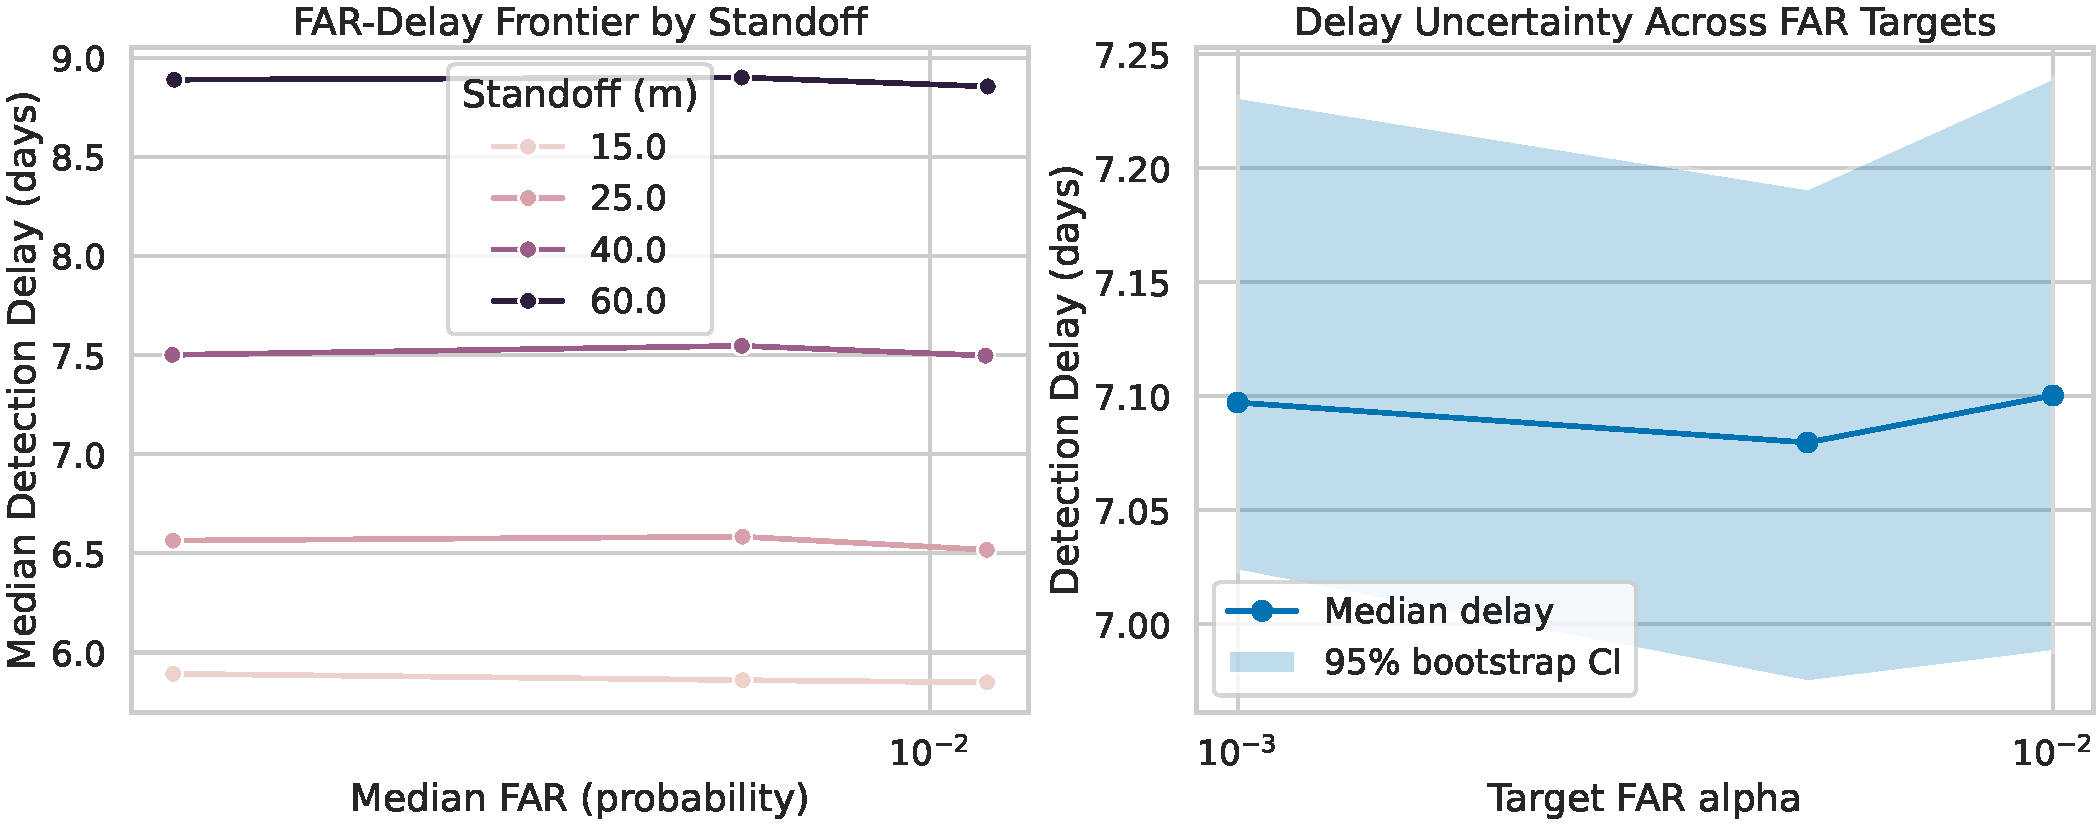
\includegraphics[width=0.67\linewidth]{figures/exp_ed_01_far_delay_frontier.pdf}
\caption{Performance frontier for the robust detector under matched operating points. Panel (A) presents median false-alarm versus delay behavior across standoff settings, while panel (B) reports 95\% bootstrap intervals for delay across FAR targets. The figure shows that stricter operating points increase delay in a controlled monotonic pattern and that uncertainty bands remain narrow enough to support comparative interpretation rather than only qualitative trend reading.}
\label{fig:frontier}
\end{figure}

Table~\ref{tab:acceptance} reports core acceptance metrics. The delay criterion is strongly satisfied: the robust method beats the single-prior baseline in $99.65\%$ of evaluated slices. However, calibration and leave-one-prior-out stress checks fail by wide margins, indicating that robust delay gains are not yet equivalent to robust calibration closure.

\begin{table}[t]
\caption{Acceptance-check summary for the executed benchmark. The first row confirms broad delay robustness at matched operating points. The remaining rows show why calibration and transfer claims are currently conditional: FAR-control stress thresholds were exceeded in contradiction-prior and leave-one-prior-out slices.}
\label{tab:acceptance}
\centering
\small
\renewcommand{\arraystretch}{1.1}
\setlength{\tabcolsep}{4pt}
\begin{tabular}{lcc}
\hline
Metric & Observed value & Target \\
\hline
Delay win rate vs single-prior baseline & 0.9965 & $\ge 0.70$ \\
Calibration violation rate & 0.9524 & $\le 0.05$ \\
Leave-one-prior-out FAR inflation (95th pct.) & 1.2871 & $\le 1.25$ \\
Median delay ratio (robust vs fixed-threshold TS) & 0.6943 & $<1.0$ desirable \\
Transfer degradation ratio (hard/easy regimes) & 1.5402 & $\le 1.25$ desirable \\
\hline
\end{tabular}
\end{table}

\subsection{Prior-Specific Calibration and Transfer Behavior}
\Figref{fig:transfer} exposes where robustness degrades. The hardest slices combine high drift with long standoff, and conservative prior-family settings carry the largest FAR inflation pressure. This aligns with the contradiction map from the literature phase: when source priors diverge, threshold conservatism can still fail in out-of-family or high-misspecification regions even if nominal delay remains strong.

\begin{figure}[t]
\centering
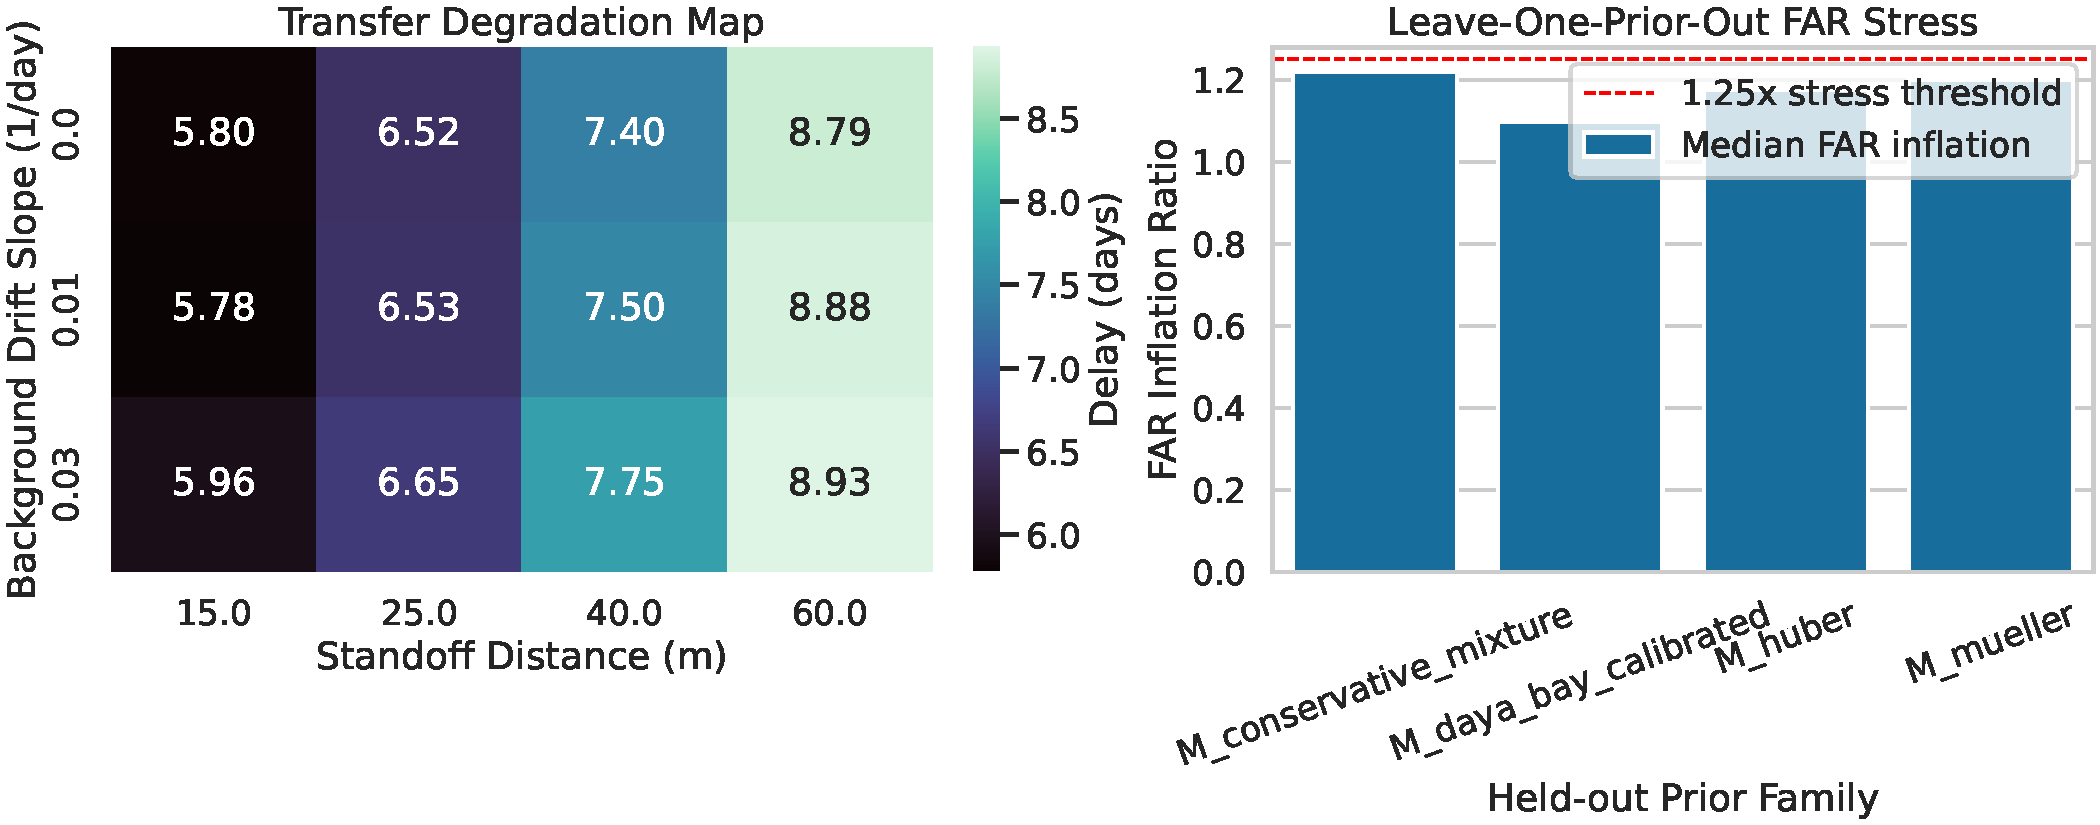
\includegraphics[width=0.67\linewidth]{figures/exp_ed_01_transfer_degradation.pdf}
\caption{Transfer-stability diagnostics for stress regimes and prior families. Panel (A) maps degradation across drift and standoff settings and identifies worst-case concentration in jointly difficult regions, while panel (B) summarizes leave-one-prior-out FAR inflation by prior family against the stress threshold. The figure indicates that transfer instability is structured rather than random, which is useful for targeted recalibration experiments but also confirms that current robustness closure is incomplete.}
\label{fig:transfer}
\end{figure}

Table~\ref{tab:prior_cal} provides prior-family slices. One prior family is materially better (calibration violation rate $0.8097$ and FAR inflation $1.183$), while three remain at violation rate $1.0$ with inflation beyond tolerance. This heterogeneous pattern is informative: it supports contradiction-aware adaptation rather than one-size-fits-all calibration.

\begin{table}[t]
\caption{Prior-family calibration diagnostics for the robust method. Differences across prior families are substantial, with one family approaching stress tolerance while others remain above it. The table supports a conditional interpretation: robust calibration is promising but not uniformly closed across contradiction-aware prior sets.}
\label{tab:prior_cal}
\centering
\small
\renewcommand{\arraystretch}{1.1}
\setlength{\tabcolsep}{4pt}
\begin{tabular}{lccc}
\hline
Prior family & Calib. violation rate & FAR inflation (95th pct.) & Median delay (days) \\
\hline
Conservative mixture & 1.0000 & 1.3189 & 7.41 \\
Daya-Bay calibrated & 0.8097 & 1.1830 & 6.58 \\
Huber lineage & 1.0000 & 1.2680 & 7.08 \\
Mueller lineage & 1.0000 & 1.2937 & 7.25 \\
\hline
\end{tabular}
\end{table}

\subsection{Formal Audit Outcomes and Claim Status}
All symbolic theorem checks passed, including monotonicity and LR/TS identity for calibration, information decomposition inequality for MDS improvement, and stability-bound verification for co-design. These checks strengthen formal consistency but do not override empirical failures; they only verify that claimed mathematical properties were implemented and tested coherently.

Taken together, evidence supports a nuanced claim structure. The detectability-improvement claim is supported under matched operating points and tested open-parameterized assumptions. The robust calibration and transfer-stability claims are mixed because stress criteria are violated in a nontrivial subset of regimes, including 407 FAR-inflation contradiction slices (14.13\% of robust-method runs). This mixed outcome is a strength of the reporting protocol, not a weakness: it prevents overclaiming and directly informs next experiments.

\section{Cross-Claim Synthesis and Operational Interpretation}\label{sec:synthesis}
\subsection{How Formal and Empirical Evidence Interact}
The executed evidence provides a useful example of why hybrid manuscripts should not collapse formal and empirical channels into a single confidence label. Theorems establish what must hold if assumptions are satisfied; simulations establish whether those assumptions are adequate in the tested domain and whether performance survives stress conditions. In this study, symbolic checks support the internal logic of all three formal components, but empirical closure differs by claim class. Detectability gains are robust under matched operating points, while calibration and transfer closure remain incomplete in difficult nuisance regimes.

This divergence is scientifically informative. If theorem checks had failed, the method itself would be suspect. Instead, theorem checks pass and failures concentrate in stress slices, indicating that the method family is coherent but the calibration policy and transfer envelope require refinement. That is a different conclusion from both optimistic overclaiming and blanket rejection. It also matches the contradiction map inherited from prior phases: unresolved source-prior disagreement can preserve useful detector ranking behavior while still widening threshold risk tails.

The distinction also clarifies how to interpret mixed support. A mixed status does not mean the claim is false; it means the claim does not yet hold at the requested robustness level across the tested stress envelope. This interpretation keeps the research trajectory constructive. One can preserve supported subclaims (for example, delay robustness under matched operating points) while narrowing unresolved claims to explicit conditions and follow-up checks.

\subsection{Decision-Theoretic Consequences for Safeguards Use}
From an operations perspective, the key tradeoff is between early-warning speed and alarm credibility. Delay improvements matter because delayed response can erase practical intervention windows. However, false-alarm inflation can overwhelm operations with low-value alerts and can reduce trust in the monitoring channel. The current results suggest that the robust method is already valuable for sensitivity-oriented screening, but not yet sufficient for autonomous decision triggers in high-consequence settings.

A practical deployment strategy implied by these findings is staged use. In stage one, the robust detector serves as a sensitivity-preserving triage layer under transparent caveats, prioritizing missed-event reduction. In stage two, a recalibrated or secondary confirmatory layer applies stricter prior-family adaptation and transfer-aware constraints before high-consequence escalation. This staged policy is consistent with the mixed evidence profile and avoids forcing a single detector policy to satisfy incompatible objectives in one step.

The observed prior-family heterogeneity supports this staged approach. A family near stress tolerance can be used to initialize conservative thresholds, while high-inflation families can trigger adaptive correction or additional evidence requirements. Importantly, this does not violate fairness, because operating-point matching remains enforced throughout comparator evaluation. Instead, it transforms contradiction-aware priors from a source of uncertainty into a structured control signal for calibration policy.

\subsection{Contradiction Map Reconciliation in the Present Study}
The literature contradiction map highlights three unresolved tensions: anomaly attribution disagreement, variable gain from shape information under calibration drift, and uncertain transfer from reactor-domain evidence to fusion-adjacent settings. The present manuscript resolves these tensions partially and explicitly. It resolves the second tension enough to support detectability gains, because count-shape integration improves delay under matched operating points in the executed benchmark. It does not fully resolve the first and third tensions, because calibration and transfer stress criteria are not met globally.

This partial reconciliation is still progress. It converts abstract contradiction into measurable closure targets, each with an associated metric threshold and evidence artifact. In practical terms, it means the field can iterate on the unresolved dimensions without reopening already supported components. Methodologically, this is superior to all-or-nothing narratives because it preserves usable knowledge and shortens subsequent iteration cycles.

\subsection{Boundary of Valid Inference}
The manuscript's inference boundary is intentionally strict. Claims are valid for open, parameterized scenarios with explicit nuisance ranges and matched-FAR comparator policy. Claims are not currently valid as plant-specific guarantees in proprietary fusion operations or as universal calibration guarantees across unbounded prior misspecification. This boundary is repeated across methods, results, and limitations to avoid scope drift.

Maintaining this boundary also improves portability. Other groups can reuse the formal definitions, robustness operators, and claim-audit protocol in adjacent monitoring domains even when domain-specific priors differ. In that sense, the most transferable product of this work is not a single parameter setting; it is a reproducible evidence discipline that ties theorem assumptions, stress-test outcomes, and caveats into one coherent decision record.

\subsection{Implications for Next Iteration Design}
The synthesis above determines concrete next-iteration priorities. First, calibration redesign should be targeted where the current method fails most often: high-drift and long-standoff slices under conservative prior-family stress. Second, transfer robustness should be optimized as an explicit objective term rather than left as a post-hoc diagnostic. Third, contradiction-aware adaptation should be tested with leave-one-prior-out constraints in the training objective itself, not only in evaluation.

These priorities are not speculative add-ons. They are the minimum changes needed to move mixed claims toward supported status under the same evidence policy used in this manuscript. Because the current framework already logs contradiction slices and symbolic outcomes, these follow-up experiments can be executed as true deltas rather than full pipeline rewrites.

\section{Discussion}\label{sec:discussion}
The central practical insight is that robust detection and robust calibration are different achievements. The benchmark demonstrates strong delay robustness relative to non-minimax baselines, which is encouraging for early warning. Yet the same benchmark shows that calibration under prior contradiction can fail exactly where transfer risk is highest. In safeguards practice, this distinction matters because a detector that is fast but poorly calibrated can produce unacceptable operational burden.

A second insight is methodological. Separating count and shape channels with explicit MDS criterion is not merely theoretical decoration; it yields a concrete ranking logic for material-informed monitoring. The observed median delay-ratio improvements are consistent with the theorem-level prediction that positive shape information should improve detectability. However, the theorem is conditional on assumptions (including approximation quality and positive information decomposition), so empirical stress auditing remains mandatory.

A third insight concerns transferability. Performance collapse is concentrated in structured nuisance regions rather than uniformly distributed over the matrix. This suggests that adaptive calibration and regime-aware policies can target identifiable failure fronts instead of globally tightening thresholds and sacrificing sensitivity everywhere. The data therefore support a refinement path, not a dead end.

Finally, the paper illustrates why source-provenance discipline matters in cross-domain settings. Borrowed reactor-domain equations are reliable for constructing open parameterized studies, but fusion-adjacent deployment claims require stronger external data. Keeping this boundary explicit preserves scientific credibility and makes the manuscript useful for both method developers and domain decision-makers.

\subsection{Comparison to Conventional Evaluation Narratives}
A common narrative in monitoring papers is to report a single aggregate metric and rank methods by that value. For exploratory work this can be acceptable, but for safeguards-style decision problems it is insufficient because costs are asymmetric: missed events, false alarms, and delayed detection have different operational consequences. The present manuscript therefore uses multi-objective reporting and stress-sliced diagnostics rather than one-score ranking. This decision increases reporting complexity, but it prevents hidden tradeoffs from being misread as universal gains.

Another conventional narrative is to treat negative outcomes as peripheral exceptions. Here, negative outcomes are central data. The 407 stress failures are not noise around an otherwise successful model; they define the boundary where calibration and transfer claims stop being globally valid. This boundary-centered reporting style is particularly important when adapting reactor-domain methods to fusion-adjacent scenarios, because domain mismatch can produce brittle success if failure structure is not examined explicitly.

A third narrative difference concerns theorem usage. Formal statements are often presented either as detached theoretical sections or as proof sketches with limited integration into empirical analysis. In this work, theorem obligations were linked to explicit symbolic checks and to claim-level reporting. This linkage does not make theorems ``empirically proven,'' but it does make implementation consistency auditable. For applied settings, that auditability is often more valuable than standalone asymptotic elegance.

Finally, comparator fairness is treated as a first-class scientific variable rather than a technical detail. Matched operating-point policy avoids a known source of optimistic bias in detection benchmarking. When fairness is enforced, some apparent gains shrink and some become stronger. This is not a downside; it is exactly the information required for trustworthy method comparison in high-consequence monitoring.

\section{Limitations and Future Work}\label{sec:limitations}
This study has four major limitations. First, scenario evidence is synthetic and open-parameterized; we do not have proprietary plant-specific fusion operational logs. This data gap limits external validity for policy-grade deployment claims. Second, anomaly-prior contradiction remains unresolved at the source level, so robust calibration may still be conservative in some slices and insufficient in others. Third, local asymptotic approximations used in MDS derivation can degrade in low-count or heavy-tail conditions. Fourth, the robust objective uses fixed scalarization weights; alternative mission priorities can reorder candidate rankings.

These limitations directly affect conclusions. The supported detectability result should be interpreted as an open-scenario robustness signal, not as a guarantee of turnkey deployment performance in proprietary facilities. Likewise, mixed calibration and transfer outcomes should be treated as evidence for targeted redesign rather than as proof of method invalidity.

\subsection{Future Work}
Follow-up experiments should prioritize the identified data and calibration gaps. First, adaptive two-stage calibration should be tested: a global minimax guardrail followed by prior-family correction constrained by monotonic FAR envelopes. Second, transfer-stability penalties should be integrated into the co-design objective and evaluated against the same matched-FAR policy. Third, external validity should be strengthened by cross-engine checks against independent transport workflows and, when accessible, partially shared operational traces. Fourth, negative-result partitions should be expanded into regime-conditioned diagnostics that separate drift effects from resolution and standoff effects.

Completion criteria for future closure are explicit: calibration violation rate at or below $0.05$, leave-one-prior-out inflation at or below $1.25$, and hard-regime transfer degradation at or below $1.25$ under matched operating points. Until those criteria are met, robustness claims should remain conditional.

\section{Conclusion}\label{sec:conclusion}
We presented a contradiction-aware, formally audited, and empirically executed framework for antineutrino-based detectability analysis in fusion-adjacent safeguards scenarios. The paper contributes three theorem-backed method elements: robust threshold existence with conservative control, information-decomposed MDS improvement criterion, and finite robust co-design with bounded stability. Executed evidence shows strong delay robustness and supported detectability improvement under matched operating points, but also reveals unresolved calibration and transfer-stability gaps in stress regimes.

The main scientific contribution is therefore twofold: a defensible formal structure for robust monitoring under prior contradiction, and a transparent claim-evidence protocol that reports both gains and failure modes. This balance is necessary for progressing from exploratory cross-domain modeling toward reliable safeguards decision support.

Beyond this specific application, the paper demonstrates a reusable pattern for high-consequence monitoring research: keep prior disagreement explicit, define objective functions and feasible sets before claiming optimality, enforce fair operating-point comparisons, and report unsupported edges as first-class outcomes. That pattern is portable to other domains where low-observability sensing, uncertain physical models, and asymmetric decision costs intersect. In future cycles, the same pattern can absorb stronger data sources without rewriting the methodological spine, enabling cumulative progress rather than disconnected benchmark snapshots.

\clearpage\phantomsection\label{sec:end_of_main}
